\subsection{The shortcut approach}
\label{chap:shortcut_approach}

After the problem with layers crossed our path in the first attempt, we took a step back and tried to reevaluate our approach.
The second attempt is based on looking at elements of alternatives (parser rule references) and asking: "which concepts could be inserted in this place?".
Consider again the \parserrule{content} rule and its child rules:

\begin{antlr}
	\parserrule{content}    :   \lexerrule{TEXT}
           |   \parserrule{element}
           |   \parserrule{comment}
           |   \lexerrule{CDATA}
           ;

	\parserrule{element}    :   \literal{<} \lexerrule{Name} \parserrule{attribute}* \literal{>} \parserrule{content}* \literal{</} \lexerrule{Name} \literal{>}
           |   \literal{<} \lexerrule{Name} \parserrule{attribute}* \literal{/>}
           ;

	\parserrule{comment}    :   \literal{<!--} \lexerrule{TEXT} \literal{-->} ;
\end{antlr}

We started building on top of the algorithm mentioned in \ref{chap:straight_algorithm}.
This leaves us again with a concept for each alternative and an interface for parser rules containing more alternatives.
We can see that the content rule can ultimately expand into following concepts:

\begin{itemize}
	\itemsep0em
	\item \textbf{Content{\_}1} (TEXT)
	\item Content{\_}2 $\rightarrow$ \textbf{Element{\_}1}
	\item Content{\_}2 $\rightarrow$ \textbf{Element{\_}2}
	\item Content{\_}3 $\rightarrow$ \textbf{Comment}
	\item \textbf{Content{\_}4} (CDATA)
\end{itemize}

The layer problem (\ref{chap:layer_problem}) dwells in the need of inserting the \concept{Content{\_}2} concept before being able to insert one of the \concept{Element{\_}1} or \concept{Element{\_}2} concepts.
We would like to avoid that and offer directly the concepts that are at the end of the chain (in bold).
These are concepts we would like to see in the auto-completion menu.
They cannot transparently break into more rules and for the sake of text we will call them \textbf{end concepts}, or when talking about the grammar rule tree \textbf{end rules}.
\\

We will describe an algorithm, that will find all end rules for a given parser rule, and later utilize it.

\subsubsection{The algorithm}
To find end rules for each parser rule, we can recursively scan through the parser tree, that we have built before.
For each parser rule, we will try to find paths leading to some end rule through its alternatives:

\begin{itemize}
	\item Whenever we find an alternative, that contains only one element, and this element is a reference to another parser rule, we have found an intermediary level that can be transparently hidden from the user of the language.
	We will continue recursively processing alternatives of this “level” rule (we are not at the end of the chain yet).

	\item Otherwise, we have found an end rule (recursion stops here).
\end{itemize}

We have expressed this algorithm using a pseudo-code:

\label{chap:shortcut_algorithm}
\begin{antlr}
	FindPathsToEndNodes(\parserrule{R}):
	1)  Define \parserrule{L} as an empty list of list of nodes
	2)  Return FindPathsToEndNodes(\parserrule{R}, \parserrule{L})

	FindPathsToEndNodes(\parserrule{R}, \parserrule{L}):
	3)  Define \parserrule{Q} as list of list of nodes
	4)  For each alternative \parserrule{A} of rule \parserrule{R}:
	5)      \parserrule{L1} = Clone(\parserrule{L})
	6)      If \parserrule{A} is a parser rule with only one element \parserrule{E}:
	7)          Let \parserrule{I} be interface/concept representing rule \parserrule{E}
	8)          \parserrule{L1}.Add(\parserrule{I})
	9)          \parserrule{P} = FindPathsToEndNodes(\parserrule{E}, \parserrule{L1})
	10)          \parserrule{Q} = Merge(\parserrule{Q}, \parserrule{P})
	11)      Else
	12)          \parserrule{L1}.Add(\parserrule{R})
	13)          Let \parserrule{P} be concept representing \parserrule{A}
	14)          \parserrule{L1}.Add(\parserrule{P})
	15)          \parserrule{Q}.Add(\parserrule{L1})
	16)  Return \parserrule{Q}
\end{antlr}

By appending the rule that is leading to current element (line 12) and then appending that alternative's element itself (line 14), we will get a path that contains the full path and the target end rule as the last element of the chain.
The result of this algorithm, for example for the \parserrule{content} rule, equals the listing of the five paths mentioned in the beginning of this chapter.
\\

We can do this for all parser rules and for each rule we will get a list of paths that lead from that particular rule to an end node.
We will call these paths \textbf{shortcuts}, as they can provide a shortcut from the rule to the end of the chain.
Now that we have these, we will talk about several ways, how to use them to make our language better.

\subsubsection{Smart auto-completion}
The first attempt on how to use shortcuts (the result of the algorithm in \ref{chap:shortcut_algorithm}) was built on top of the previous approach.
There were no structural changes when it came to interfaces or linking concepts together.
We imported everything just the same and then added some more functionality.
\\

We were trying to solve the most obvious problem in front of us --- the auto-completion.
We would like to improve it so that it offers us only end concepts.
Luckily for us, MPS gives us the ability to create custom auto-complete menus and use those instead of the built-in one.
This means, that we are going to be able to construct our own menu containing only end nodes.
Unfortunately, it requires us to implement some non-trivial mechanisms.

\paragraph{Defining the auto-complete}

The auto-complete menu is bound to a cell of the projectional editor containing a reference to one of the children of a concept.
Let's say we are again talking about the concept that represents the element rule's first alternative.
As described above earlier in the process (\ref{fig:element_concept_full}), we created:

\begin{itemize}
	\item An interface \interface{IContent} representing four different alternatives that the content rule can break into

	\item A child of the \concept{Element{\_}1} concept, that references the \interface{IContent} rule
\end{itemize}

Somewhere in the editor aspect of the \concept{Element{\_}1} concept, there will be a cell referencing the concept interface \interface{IContent}.
The cell, together with the auto-complete property can be seen in figure \ref{fig:autocomplete_cell}.
\\

\begin{figure}[h]
	\centering
	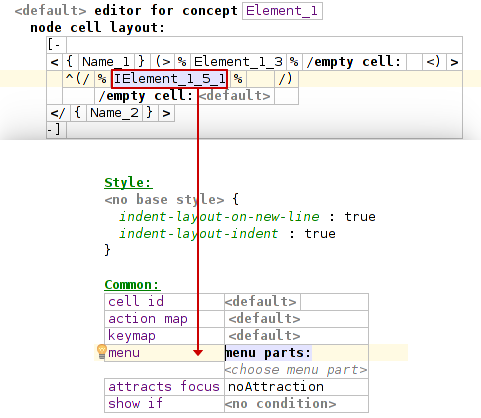
\includegraphics[scale=0.7]{./img/autocomplete_cell.png}
	\caption{Auto-complete property}
	\label{fig:autocomplete_cell}
\end{figure}

We would like to create an auto-complete for this cell, that would contain following options (end concepts):

\begin{itemize}
	\itemsep0em
	\item Content{\_}1
	\item Element{\_}1
	\item Element{\_}2
	\item Comment
	\item Content{\_}4
\end{itemize}

Because we are inside MPS everything is a concept node.
In order to create an auto-complete menu, we need to create some BaseLanguage node and put it inside some AST (referencing the menu).
More precisely, we will create an instance a concept called \texttt{CellMenuPart{\_}ReplaceChild{\_}CustomActionConcept}, contained in one of many MPS's core languages.
\\

For this concept, we will define a number of auto-complete options, one for each end concept, that we want to offer in the menu.
Every option has a \textbf{textual description}, \textbf{matching text} (so that we can filter through them) and most importantly a \textbf{creator method}.
If the user selects that particular option, this method will be called with some contextual information in parameters and it is expected to return an instance of some concept that implements the \interface{IContent} interface.
\\

The complicated part of the process comes now, as we would like to dynamically generate the creator method.
We need to create BaseLanguage statements, that will instantiate the end concept and return it.
There is one small problem, though.
Let's say the user selected the second option and decided to insert another \concept{Element{\_}1} inside.
The problem is, that \concept{Element{\_}1} doesn't implement the \interface{IContent} interface.
It only implements the \interface{IElement} interface as per the algorithm of the straightforward approach (\ref{chap:straight_algorithm}).
The shortcut, that leads to this end concept leads through the \concept{Content{\_}2} concept, that has an Element child.
This means, that we have to follow the whole path and chain individual nodes, beginning with the \concept{Content{\_}2} concept.
For this particular case it would mean to:

\begin{itemize}
	\item Create an \concept{Element{\_}1} concept and store it in a variable.

	\item Create a \concept{Content{\_}2} concept and store it in a variable.

	\item Assign the \concept{Element{\_}1} node to the right child of the \concept{Content{\_}2} node.

	\item Return \concept{Content{\_}2} node.
\end{itemize}

As we said earlier in section \ref{chap:generating_code_inside_mps}, generating BaseLanguage code is a bit more complicated because we need to either use a quotation or create a large number of AST nodes.
Using a quotation, in this case, was sometimes impossible as everything is very dynamic.
The finished option concept is shown in figure \ref{fig:autocomplete_action}.

\begin{figure}[h]
	\centering
	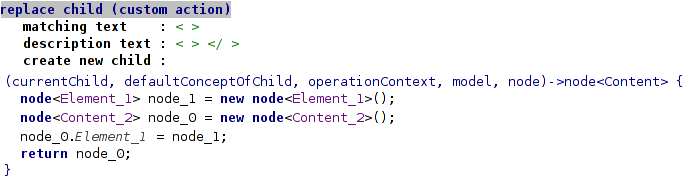
\includegraphics[width=\textwidth]{./img/autocomplete_action.png}
	\caption{Auto-complete action code (Element{\_}1 concept)}
	\label{fig:autocomplete_action}
\end{figure}

For the description text we used concept's alias.
We talk about creating aliases in section \ref{chap:common_ground}.
For matching text we used the shortest unique prefix of alias among all other options' aliases in given auto-complete menu.
The algorithm for searching shortest unique prefixes in a set of strings is not important from our thesis' point of view, so we decided to not go into further detail.


\paragraph{The layer problem again}

After we implemented the auto-complete menu, coding in the imported language started to be very reasonable and comfortable, since we eradicated intermediate layers.
Or did we?
When producing code, the language really does what one would expect.
However, when the user starts deleting code, the layer problem occurs once more.
\\

What happens here is, that when we select the auto-complete option, several layers of concepts might get created and inserted into the cell.
Imagine, we just inserted the \concept{Element{\_}1} node.
According to the creator method, this new node is wrapped inside of the \concept{Content{\_}2} node.
Now let's say, the user changed his mind, and wants to replace this XML element with a comment.
He would press backspace, the XML element would disappear as expected.
Then, the user continues by invoking the auto-complete menu again, expecting to have all five options at hand.
What happened instead is that the \concept{Element{\_}1} node got deleted, but the wrapping \concept{Content{\_}2} one remained.
The \concept{Content{\_}2} concept has only one child of type Element and that is why our user only sees \concept{Element{\_}1} and \concept{Element{\_}2} as options in the auto-complete.


\paragraph {The deletion context}

Solution to this resurrected layer problem lies in controlling the deletion event.
Once again, MPS' authors have equipped us with tools for doing this.
We are able to specify our own handler for the deletion event for any cell of the projectional editor.
But what will it look like?
\\

When deleting a node, we would like to remove the whole shortcut path, effectively reversing the effect of the creator method.
We decided that it will be the easiest to store the length of the path, that is leading to certain AST node, together with the node.
So when we are creating nodes, while building the path in the creator method, we tell each node, how deep or far on the path the node is.
In order to do this, we created a \concept{BaseConcept}, a parent abstract concept, from which we will inherit all other concepts.
This abstract concept will define a special integer property, that will hold our information, effectively making all other concepts inherit it too.
We called this property \textit{{\_}{\_}DeleteContext} and enhanced the creator method as shown in figure \ref{fig:autocomplete_action_delete_context}.

\begin{figure}[h]
	\centering
	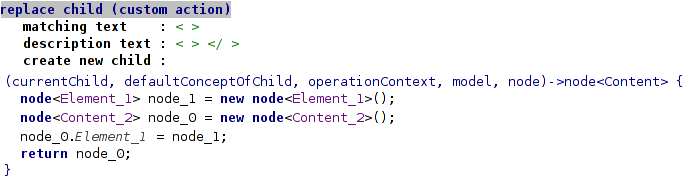
\includegraphics[width=\textwidth]{./img/autocomplete_action_delete_context.png}
	\caption{Auto-complete action extended with deletion context}
	\label{fig:autocomplete_action_delete_context}
\end{figure}

The last thing remaining, is creating the backspace action.
Apart from some problems with referencing the \textit{{\_}{\_}DeleteContext} property, which must be reached through the abstract \concept{BaseConcept} type, it is quite straightforward to generate a BaseLanguage code like shown below (figure \ref{fig:backspace_action}).

\begin{figure}[h]
	\centering
	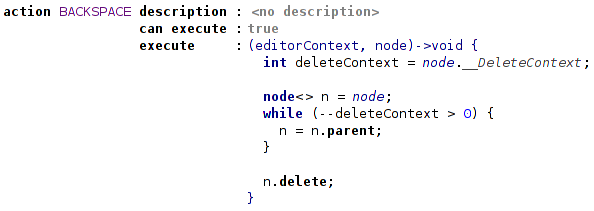
\includegraphics[width=\textwidth]{./img/backspace_action.png}
	\caption{Backspace action implementation}
	\label{fig:backspace_action}
\end{figure}

We must not forget to pin this handler to every cell, that we pin the auto-complete menu to.
After we had done this, the layer problem has finally been eradicated.
The language became a bit more usable once more.

\subsubsection{Smart interfaces}

After we have implemented the smart auto-complete, we realized, that there might be another way to accomplish almost the same result.
It would mean changing the first step concerning interfaces and concept linking.
\\

The main idea behind this is the realization, that if for each concept interface there exists a finite set of end concepts, we could just create a special interface and let all these and only these end concepts implement it.
It is important, that other non-end concepts, that are in the shortcut path, will not implement it.
Otherwise, that would put us right back where we started with the straightforward approach \ref{chap:straightforward_approach} and the layer problem \ref{chap:layer_problem}.
To give an example regarding our content rule, we would create an \interface{IContent} interface concept and only following concepts would implement it:

\begin{itemize}
	\itemsep0em
	\item Content{\_}1
	\item Element{\_}1
	\item Element{\_}2
	\item Comment
	\item Content{\_}4
\end{itemize}

There would be no need for the \concept{Content{\_}2} concept at all.
Concepts would, of course, implement as many interfaces as many shortcuts lead to them.
The difference is, that the intermediary layers will not, which will prevent the layering.
\\

We still need to find end concepts for each rule, so we will keep the same algorithm for finding shortcuts as before.
We, however, do not need to implement our own auto-completion and, subsequently with it, no deletion handlers.
The built-in default auto-completion will start to behave exactly the same way our smart auto-completion does.

\paragraph{Cardinality restriction}
\label{chap:cardinality_restriction}

So far it looks like the last approach is superior to the auto-completion one.
It avoids complicated code generation and even resulting MPS languages are more simple and better performant, as they are not bloated with auto-completion code.
There is one small drawback, though, that makes this solution slightly suboptimal.
\\

To remind the reader --- the cardinality of an element is telling us, how many of each specific child rules can occur inside an alternative.
Inside the grammar, this was expressed using quantification operators (\textbf{*},\textbf{+} and \textbf{?}).
The problem, that appears here, can be shown using this example rule:

\begin{antlr}
\parserrule{content}      :   \parserrule{element}+
             |   \parserrule{comment}*
             |   \lexerrule{CDATA}?
             ;
\end{antlr}

Notice, how we changed the cardinality of elements inside the \parserrule{content} rule.
This small change will prevent us from creating a shortcut leading through this rule.
We are trying to say, that shortcuts, that can be used for the smart interfaces approach, can only lead through rules, that have cardinality [1..1].
This means through an alternative with a single child element, that is a reference to a parser rule AND has the [1..1] cardinality.
In the original \parserrule{content} rule, all alternatives look like this, so there was no problem.
Speaking in terms of the shortcut algorithm \ref{chap:shortcut_algorithm}, we would alter line number 6 and add this restriction to the condition.
\\

This restriction is caused by the fact that we would be unable to control changing children cardinality on the whole shortcut path.
Imagine, that some alternative of some other rule contains a reference to this altered \parserrule{content} rule (regardless of its quantitative operator).
The list of shortcuts, that will be generated for this new setup is following:

\begin{itemize}
	\itemsep0em
	\item Content{\_}1\textbf{+} $\rightarrow$ Element{\_}1
	\item Content{\_}1\textbf{+} $\rightarrow$ Element{\_}2
	\item Comment\textbf{*}
	\item Content{\_}3\textbf{?}
\end{itemize}

When we would be creating a child link holding the \interface{IContent} type, we would be setting cardinality of the child link depending on the cardinality of the \parserrule{content} reference.
But each alternative of the altered \parserrule{content} rule requires a different number of children to be inserted.
This means, that when we would follow the shortcut path and assign the \interface{IContent} interface to the \concept{Element{\_}1} and to the \concept{Element{\_}2} concept, we will lose the \textbf{+} cardinality information since we would only enable the user to insert one child of the \interface{IContent} child.
\\

A small example might demonstrate this better.
We have an \interface{IContent} [1..1] child.
If we disregarded the cardinality restriction, we could ultimately put there the \concept{Element{\_}1} end concept node.
But the content rule says, there can be [1..n] elements.
We are still bound to insert only one, though.
\\

The smart auto-completion approach mentioned above could solve this problem by generating lists of children with the corresponding cardinality.
